\chapter{Logik}

\section{Projektstruktur}

Das Projekt lässt sich in mehrere Teilmodule (Packages) aufgliedern. Gemäß dem objektorientieren Programmieren werden Klassen, die einen logischen Zusammenhang besitzen, in ein Package zusammengefasst.

\begin{figure}[!ht]
\centering
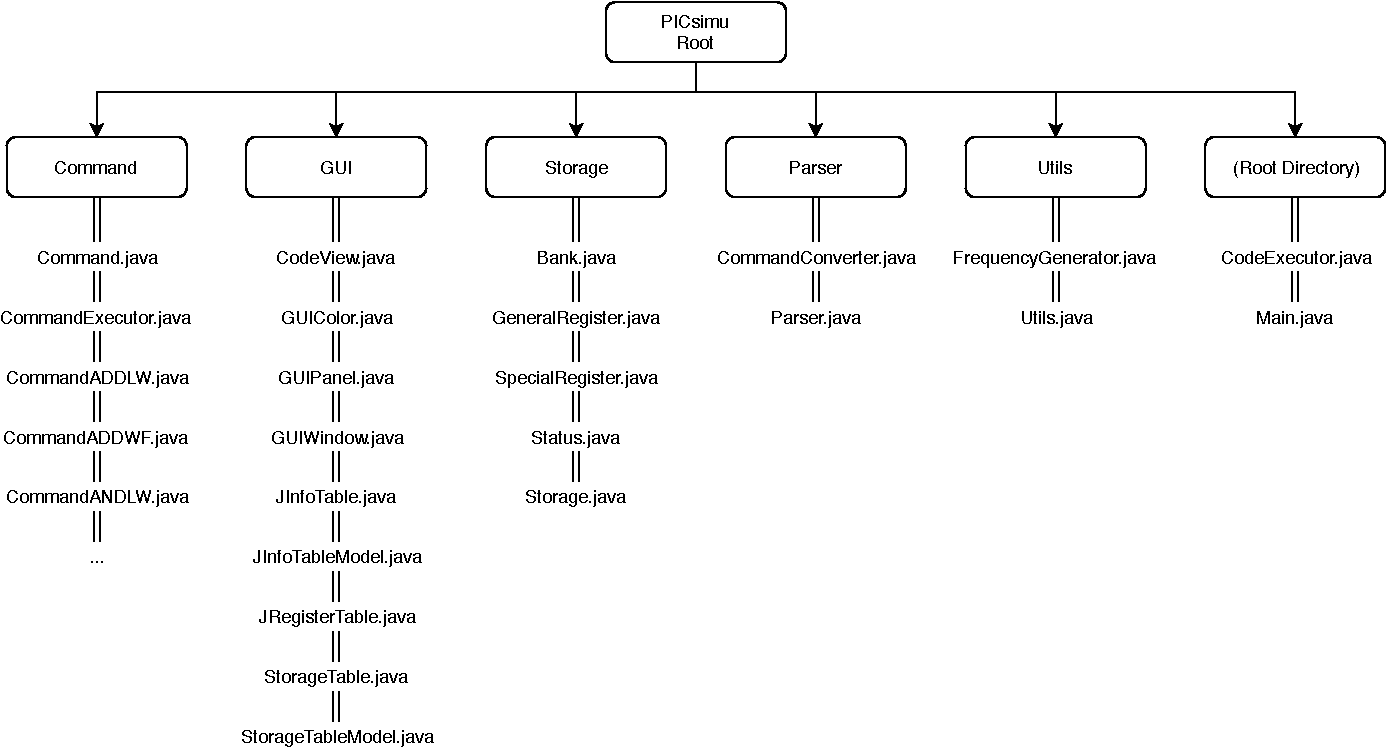
\includegraphics[width=\textwidth]{img/PICsimu-tree.pdf}
\caption{Projektstruktur-Baum}
\label{project-tree}
\end{figure}

\noindent In diesem Projekt gibt es nachfolgende Packages; es werden die darin wichtigsten Klassen erklärt.

\begin{description}
\item[Command]{Dieses Package beinhaltet die Klassen zu sämtlichen Assemblerbefehlen - von \textit{ADDLW} bis \textit{XORWF}. Zudem gibt es die Superklasse \textit{CommandExecutor} mit Methoden, welche das Status-Register nach einer Rechenoperation beeinflussen. In der Enumeration \textit{Command} werden alle Befehle aufgelistet - inklusive Befehlscode, Argumentmaske, Anzahl Quarztakte sowie die \enquote{Status Affected Bits}.}
\item[GUI]{Dieses Package beinhaltet die Klassen zur grafischen Oberfläche - dem Frontend. Das Fenster wird hierbei über die Klasse \textit{GUIWindow} erzeugt, in welcher bereits einige Einstellungsparameter (wie z.B. die Fenstergröße) festgelegt sind. Die Darstellung der gesamten Oberfläche und zugehörigen Bedienfeldern findet sich in der Klasse \textit{GUIPanel} wieder. Wichtige Komponenten sind dabei wieder in eigene Klassen ausgelagert. Die Klasse \textit{GUIColor} ist außerdem zuständig für die Farbdarstellung, damit die Dark-Mode-Einstellung das Farbschema zu einem dunkleren Farbton ändert. }
\item[Storage]{Dieses Package beinhaltet die Klassen zum (Register-) Speicher sowie zur Bankumschaltung. Die Enumeration \textit{SpecialRegister} beinhaltet eine Auflistung der Spezialregister (z.B. Status-Register) mit deren Speicheradressen und Standardbelegung. In der Klasse \textit{Storage} wird der Speicher (inklusive EEPROM) des Mikrocontrollers verwaltet.  Außerdem befinden sich hier auch das PC-Register (PCL, PCLATH und der interne ProgramCounter) und Methoden, um den Ablauf des Programms zu verändern (setPC). }
\item[Parser]{Dieses Package beinhaltet die Klassen zum Parsing der Programme für den Mikrocontroller. Die ganzen Befehle sind dabei in der Enum-Klasse \textit{Command} zusammen mit den Masken und Längen des Befehlscodes gespeichert. So wird jeder eingehende Hexcode der Quellcodedatei Zeile für Zeile ausgelesen und mithilfe der Maske einem Befehl zugeordnet. Die eingelesenen Befehle werden dann als Command mit Argument und Zeile in der Quellcodedatei gespeichert, damit eine mögliche spätere Zuordnung (bspw. für Breakpoints) stattfinden kann. }
\item[Utils]{Dieses Package beinhaltet Klassen mit nützlichen (programminternen) Hilfsmethoden sowie einen einstellbaren Frequenzgenerator, der an die Pins von PORTA bzw. PORTB angelegt werden kann.}
\item[(Root Directory)]{Dieses Package ist das Root Verzeichnis der Packages. In diesem liegen alle anderen Packages sowie die Klasse \textit{Main} und \textit{CodeExecutor}. Die Klasse Main ist der Eintrittspunkt der gesamten Anwendung. Hier wird der CodeExecutor initiiert, welcher dann das Fenster öffnet und auf Eingaben wartet. Im CodeExecutor befindet sich auch der Timer, damit Befehle automatisch nacheinander ausgeführt werden können. Der Reihe nach werden die Befehle aus dem CommandSet ausgeführt und bestimmen dadurch den Ablauf des Programms. Der Befehl GOTO verändert beispielsweise den ProgramCounter und zeigt darüber dem CodeExecutor, dass der nächste Befehl an einer anderen Stelle steht. }
\end{description}


\section{Speicherverwaltung}

Der Speicher, inklusive EEPROM, wird in der Klasse \textit{Storage} verwaltet. Im Folgenden werden die wichtigsten, öffentlichen (\enquote{public}), Methoden dieser Schnittstelle erläutert.

\begin{description}
\item[void resetAll()]{Setzt sämtliche Register, auch W-Register und Stack, auf ihre Standardwerte zurück.}
\item[void manipulatePC()]{Methode zum Verändern des PC über Registermanipulation durch Befehle. Setzt PCL, PCLATH und den PC.}
\item[void jumpPC()]{Methode zum Verändern des PC über Sprungbefehle wie CALL und GOTO. Setzt PCL und den PC.}
\item[void incrementPC()]{Methode zum Inkrementieren des PC während des Befehlsdekodierungsprozesses. Setzt PCL und den PC.}
\item[int getRegister(int address, boolean ignoreBank)]{Versucht, ein GeneralRegister oder ein SpecialRegister an der Adresse \texttt{address} zu finden. \texttt{ignoreBank} ignoriert die Bankumschaltung und wertet \texttt{address} als absolute Adresse aus. Ist \texttt{address == 0x00}, wird die reale Adresse aus dem FSR geholt. Wenn kein Register an der Adresse gefunden wurde, wird eine Java-Exception geworfen, ansonsten wird der Wert des gefundenen Registers als \texttt{int} zurückgegeben.}
\item[boolean isBitOfRegisterSet(...)]{Gibt zurück, ob ein bestimmtes Bit in einem Register gesetzt ist (\texttt{= 1}) oder nicht (\texttt{= 0}).}
\item[void setRegister(int value, ...)]{Setzt ein Register auf den Wert \texttt{value}. Weitere Parameterbeschreibung und Ablauf siehe \texttt{getRegister(...)}.}
\item[void setBitOfRegister(boolean setBit, ...)]{Setzt ein bestimmtes Bit in einem Register mit dem Parameter \texttt{setBit}.}
\end{description}
